\section{Ciencia del diseño}
Este proyecto se desarrollará bajo la metodología de la ciencia del diseño. En esta metodología se busca diseñar e investigar artefactos en un contexto específico \cite{wieringa_design_2014}. Dentro de esta metodología los artefactos son cualquier cosa que es diseñada por la persona investigadora, desde programas de software hasta técnicas. Por otra parte, el contexto es todo aquello que no puede ser diseñado por la persona investigadora, como el hardware en el que se ejecutará el programa o las restricciones de presupuesto.
En la figura \ref{fig:artifact} podemos observar la relación entre el artefacto y el contexto en nuestra investigación. El artefacto será una simulación sismológica que hace uso de la visualización y análisis in-situ que se desarrollará, mientras que el contexto incluye el hardware que tenemos disponible para ejecutar las simulaciones, los datos que tenemos disponibles, los contactos que se cuentan con sismólogos corresponde a las técnicas computacionales aplicadas a la sismología. Es importante siempre tener en cuenta el contexto mientras se realiza el desarrollo de la simulación ya que es la interacción entre ambos lo que llevará a la resolución del problema.
\begin{figure}
  \centering
  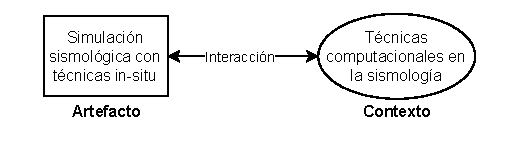
\includegraphics[width=0.9\textwidth]{artifact_context}
  \caption{Tema de investigación}
  \label{fig:artifact}
\end{figure}

\section{Actividades a realizar}
\label{sec:activities}

El marco de trabajo que se utiliza en la ciencia del diseño se presenta en la figura \ref{fig:framework}. El contexto social se refiere a aquellas personas que impactan y son impactadas por nuestra investigación. En nuestro caso las personas interesadas son investigadores en sismología, los desarrolladores de bibliotecas in-situ y los desarrolladores de la simulación sismológica SPECFEM. El contexto del conocimiento se refiere a las áreas del saber que impactan y son impactadas por el proyecto. En nuestro caso estas incluyen la sismología, las técnicas de análisis y visualización in-situ y la computación de alto rendimiento.

En la ciencia del diseño, un problema de investigación se divide en problemas de diseño y preguntas de conocimiento. Los primeros se resuelven con ciclos de diseño y los segundos con ciclos empíricos. En nuestro proyecto identificamos las siguientes partes:

\begin{itemize}
    \item Pregunta de conocimiento 1 (PC1): ¿Cuáles técnicas in-situ se utilizan en otros dominios de la ciencia a parte de la sismología?
    \item Problema de diseño (PD): La extensión de una simulación sísmica numérica para que utilice el análisis y la visualización in-situ.
    \item Pregunta de conocimiento 2 (PC2): ¿Qué tan efectiva es la herramienta desarrollada en términos de ciencia y rendimiento computacional?
\end{itemize}

El ciclo empírico (CE1) para responder la PC1 tendrá como objetivo el caracterizar simulaciones en otros dominios que hayan incorporado el análisis in-situ. Para realizar esto se llevará a cabo una revisión sistemática de literatura utilizando la guía PRISMA 2020 \cite{Page2021}. 
Las actividades relacionadas a este ciclo son las siguientes:
\newcounter{tasks}
\begin{enumerate}
    \item Definir los parámetros de la revisión: Esta actividad incluye la delimitación de la búsqueda, la creación del protocolo de revisión, la selección de bases de datos y las hileras de búsqueda y la definición de los criterios de inclusión y exclusión.
    \item Llevar a cabo la revisión: Aquí se llevará a cabo la búsqueda de los artículos científicos, así como la aplicación de los criterios de inclusión y exclusión, y la extracción de datos con el protocolo de revisión.
    \item Análisis de datos: Se analizarán los datos que extrajeron de la revisión y se llegará a conclusiones que se podrán utilizar para informar el desarrollo del proyecto actual.
    \setcounter{tasks}{\value{enumi}}
\end{enumerate}

En el ciclo de diseño (CD) para resolver el PD se extenderá la simulación SPECFEM3D para que haga uso de técnicas de análisis y visualización in-situ. Para lograr esto se hará uso del conocimiento obtenido en el CE1 para informar el diseño de la solución, así como el análisis de la base de código y consultas a los autores de la simulación y las bibliotecas de análisis y visualización in-situ.
Las actividades que se llevarán a cabo en este ciclo son:
\begin{enumerate}
    \setcounter{enumi}{\value{tasks}}
    \item Definición de escenarios: En esta actividad se definirán escenarios de simulación para poder validar el funcionamiento de la simulación antes y después de los cambios a realizar, así como su rendimiento computacional. Estos escenarios se definirán tras consultar con investigadores del Observatorio vulcanológico y sismológico de Costa Rica (OVSICORI) para conocer su criterio sobre qué podría ser relevante para ellos, así como para obtener los datos necesarios para poder llevarlos a cabo.
    \item Ejecución de escenarios con la simulación base: Se ejecutará la simulación con los escenarios definidos en la supercomputadora Polaris del Argonne National Laboratory (ANL) de EEUU y se obtendrán visualizaciones.
    \item Modificación del código fuente de SPECFEM3D: Se analizará el código relacionado con la E/S de datos para determinar la mejor forma de agregar la funcionalidad in-situ, intentando aprovechar las partes que actualmente hacen uso de ADIOS2. Se comunicará con los desarrolladores de la simulación para resolver posibles dudas que se encuentren. Se llevará a cabo la codificación de los nuevos módulos relacionados al análisis y visualización in-situ.
    \item Ejecución de escenarios con la simulación modificada: Se volverá a ejecutar la simulación con los escenarios definidos y se corroborá la correctitud funcional de los resultados y las visualizaciones, comparándolos con los resultados anteriores. 
    \setcounter{tasks}{\value{enumi}}
\end{enumerate}

Finalmente, en el segundo ciclo empírico (CE2) se responderá la PC2. Se realizarán validaciones de los resultados obtenidos con sismólogos y también se realizarán pruebas de rendimiento computacional, escalamiento fuerte y débil.

\begin{enumerate}
    \setcounter{enumi}{\value{tasks}}
    \item Validación con expertos en sismología: Se consultará con investigadores del área para validar los resultados de la simulación, así como la utilidad de la herramienta en la investigación que realizan.
    \item Pruebas de rendimiento: Se realizarán comparaciones entre el rendimiento de la simulación original y la simulación modificada para determinar el overhead introducido con la funcionalidad in-situ. Se harán pruebas de escalamiento débil y fuerte para entender los límites computacionales de la herramienta.
\end{enumerate}

De forma transversal se estará documentando el avance del proyecto.

\begin{figure}[h]
    \centering
    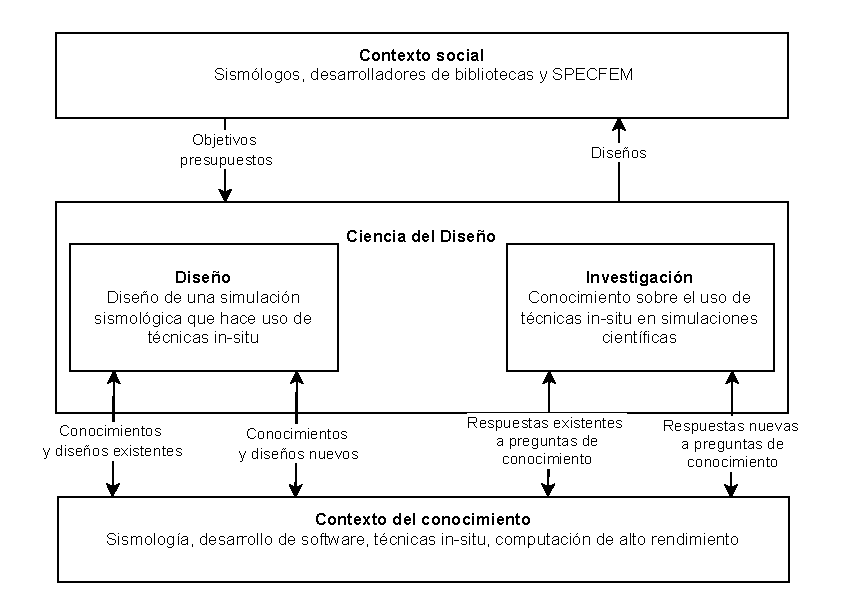
\includegraphics{framework}
    \caption{Marco de trabajo en el que se desarrolla la investigación}
    \label{fig:framework}
\end{figure}

\section{Cronograma}
Las actividades definidas en la sección \ref{sec:activities} tentativa se llevarán a cabo según el cronograma que se encuentra en la figura \ref{fig:chronogram}.

\begin{figure}
    \centering
    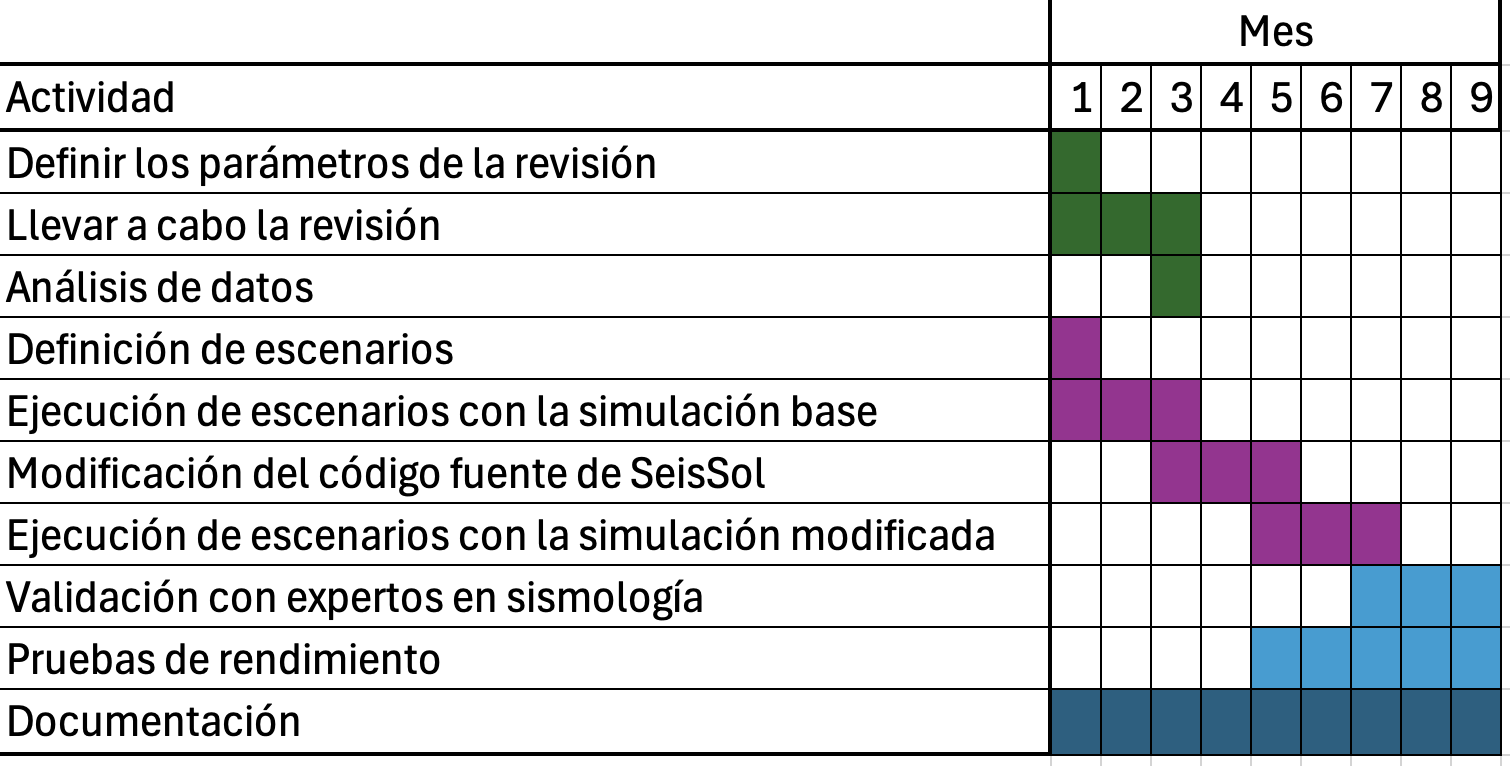
\includegraphics[width=0.7\textwidth]{chronogram}
    \caption{Cronograma tentativo para el desarrollo del proyecto.}
    \label{fig:chronogram}
\end{figure}